\documentclass[11pt,a4paper]{article}

\usepackage[T1]{fontenc}
\usepackage[utf8]{inputenc}
\usepackage{mathpazo}
\usepackage[margin=1in]{geometry}
\usepackage{amsmath,amssymb}
\usepackage{booktabs}
\usepackage{tabularx}
\usepackage{longtable}
\usepackage{siunitx}
\usepackage{xcolor}
\usepackage{enumitem}
\usepackage{graphicx}
\usepackage{caption}
\usepackage{xurl}
\usepackage[hidelinks]{hyperref}
\usepackage{cleveref}

\sisetup{group-separator={,},group-minimum-digits=4,group-digits=integer,detect-all}
\captionsetup{font=small,labelfont=bf,width=0.94\textwidth}
\setlist[itemize]{itemsep=3pt,topsep=5pt,parsep=0pt}
\setlist[enumerate]{itemsep=3pt,topsep=5pt,parsep=0pt}
\renewcommand{\arraystretch}{1.12}
\setlength{\emergencystretch}{3em}
\renewcommand{\topfraction}{0.9}
\renewcommand{\bottomfraction}{0.8}
\renewcommand{\textfraction}{0.07}
\renewcommand{\floatpagefraction}{0.75}
\setcounter{topnumber}{3}\setcounter{totalnumber}{4}

\definecolor{navy}{HTML}{1B3A6B}
\definecolor{rust}{HTML}{C1121F}

\newcommand{\okina}{\textquoteleft}
\newcommand{\Oahu}{O\okina ahu}
\newcommand{\src}[1]{\textsuperscript{[#1]}}

\title{\bfseries Which Lines Overload, and Which Neighbourhoods Lose Power\\[4pt]
\large A linear-programming reliability study of \Oahu's 138\,kV transmission grid,\\
run on one recorded year and on \num{10000} random draws}
\author{}
\date{}

\begin{document}
\maketitle
\vspace{-2.2em}

\begin{abstract}
\noindent
We rebuild \Oahu's \SI{138}{kV} transmission network from public records --- 11
substations, 16 corridors carrying 25 circuits, and the island's 24 dispatchable
generating units (\SI{1508}{MW}) --- and run one optimisation model on it: a
\textbf{linear program} that finds the cheapest way to meet every substation's demand
without pushing any line past its rating. Demand at each substation is the utility's
filed 2021 hourly island load, split between substations by census population and
jobs. Each substation's \num{8760} hourly values are summarised by a
\textbf{Gaussian distribution} --- a mean and a standard deviation --- and the eleven
Gaussians are joined by their measured correlations. We solve the program on the
\num{8760} recorded hours and on \num{10000} random hours drawn from those Gaussians,
first with every line in service and then with every single circuit (N-1) and every
pair of circuits (N-2) removed, the test the utility's own planning rule sets.

\textbf{With all lines in service, nothing goes wrong}: no line is ever more than
\SI{73}{\percent} full and all demand is served in every recorded hour and every random
draw. \textbf{Losing any one circuit still loses no demand}, but it pins the two
single circuits that carry the west side's power east (CEIP--Ewa Nui and
Kalaeloa--Ewa Nui) at their limit in \SIrange{27}{39}{\percent} of hours.
\textbf{Losing two circuits cuts power in 7 of 128 cases}: East Honolulu loses
everything if both Koolau--Pukele circuits fail; downtown Honolulu is short in
\SI{99}{\percent} of hours if two of its three supply circuits fail; Wahiaw\=a and the
North Shore are short in \SI{37}{\percent} of hours if both of their lines fail; and
the windward side with East Honolulu is short in \SI{8}{\percent} of hours if two of
the three lines into Koolau fail. Three of these --- East Honolulu, downtown and the
windward side --- are the weak spots the utility itself described to the Hawai\okina i
Public Utilities Commission in 2007. The random draws agree on every one of them and add
three rare cases (at most \SI{0.33}{\percent} of draws) that the recorded year never
produced, because the Gaussian produces demands, and mixes of demands, that the
recorded year never had. Because the substation split is built from three island-wide
sector curves, its covariance matrix is singular; giving every substation its own
independent local variation makes it full rank and leaves these answers in place,
except that Pearl Harbor becomes exposed in the recorded year too.
\end{abstract}

\vspace{0.4em}
\hrule
\vspace{1.0em}

\paragraph{How to read this paper.} Every number the model uses is either
\emph{measured} (taken from a public record of \Oahu's own grid) or a
\emph{stand-in} (taken from the closest documented source when \Oahu's own value is
not public). Stand-ins are marked where they are used, and
\cref{app:sources} lists every input with its source. Sources are cited with short
tags such as \src{HIFLD} or \src{PUC}; the tags are resolved in the reference list.

%======================================================================
\section{The optimisation problem, and the network it runs on}
\label{sec:model}
%======================================================================

\subsection{What is being decided}

Every hour, the grid operator answers one question: \emph{which power stations run,
and how hard?} Many answers keep the lights on, and they cost different amounts. The
job is to find the cheapest one that is physically legal.

Think of the network as reservoirs joined by pipes. Three rules apply.

\begin{description}[leftmargin=1.5em,style=nextline]
  \item[Nothing is stored.] At each substation, power in equals power out, in the same
        instant.
  \item[You cannot steer the flow.] How much power goes down each line is not a choice.
        It is set by the difference in voltage phase angle between the two ends --- the
        electrical equivalent of a pressure difference. Water takes every open pipe at
        once, in proportion to how easy each pipe is; so does power.
  \item[Every pipe has a width.] Each line has a rating in megawatts. Its flow, in
        either direction, must stay inside it.
\end{description}

\subsection{The variables}

\begin{center}
\small
\begin{tabular}{@{}llp{0.58\textwidth}@{}}
\toprule
\textbf{Symbol} & \textbf{Units} & \textbf{What it is, and its physical picture} \\
\midrule
\multicolumn{3}{@{}l}{\textit{Given to the model --- fixed numbers}}\\
$d_n$ & MW & the demand at substation $n$ this hour: how much water the town at
  reservoir $n$ drinks. \emph{This is the only input that changes between
  experiments.} \\
$\bar p_g$ & MW & the maximum output of generator $g$: the size of its pump \\
$c_g$ & \$/MWh & the running cost of one megawatt-hour from generator $g$ (fuel plus
  variable maintenance): what each pump charges per litre \\
$b_\ell$ & per unit & the susceptance of line $\ell$: how \emph{easy} the pipe is. A
  short line, or several circuits side by side, is a wide, short pipe with a large
  $b_\ell$ \\
$\bar F_\ell$ & MW & the thermal rating of line $\ell$: the most the pipe can carry
  before it overheats \\
$V$ & \SI{10000}{\$/MWh} & the penalty for each megawatt-hour of demand that is not
  served --- a fine so large that the model will run every pump on the island before
  it lets a town go dry\src{MISO} \\
\midrule
\multicolumn{3}{@{}l}{\textit{Chosen by the model --- the decision variables}}\\
$p_g \ge 0$ & MW & how hard generator $g$ is run \\
$\theta_n$ & radians & the voltage phase angle at substation $n$: the water level in
  reservoir $n$ \\
$s_n \ge 0$ & MW & demand that cannot be served at substation $n$ --- the town that
  goes without \\
\midrule
\multicolumn{3}{@{}l}{\textit{Follows from the above}}\\
$F_\ell$ & MW & the flow on line $\ell$ \\
\bottomrule
\end{tabular}
\end{center}

With 11 substations and 24 generators the program has $24 + 11 + 11 = 46$ decision
variables.

\subsection{The linear program}

\begin{equation}
\min_{p,\,\theta,\,s}\quad
\underbrace{\sum_{g} c_g\, p_g}_{\text{running cost}}
\;+\;
\underbrace{V \sum_{n} s_n}_{\text{penalty for unserved demand}}
\label{eq:obj}
\end{equation}
subject to, for every substation $n$ and every line $\ell$:
\begin{align}
F_\ell &= 100\, b_\ell \left( \theta_{f(\ell)} - \theta_{t(\ell)} \right)
  && \text{\small flow follows the angle difference} \label{eq:dc}\\[2pt]
\sum_{g \text{ at } n} p_g \;+\; s_n
  \;-\!\!\!\sum_{\ell \text{ out of } n}\!\!\! F_\ell
  \;+\!\!\!\sum_{\ell \text{ into } n}\!\!\! F_\ell &= d_n
  && \text{\small power in $=$ power out} \label{eq:bal}\\[2pt]
-\bar F_\ell \;\le\; F_\ell &\;\le\; \bar F_\ell
  && \text{\small the line's rating, both directions} \label{eq:lim}\\[2pt]
0 \;\le\; p_g &\;\le\; \bar p_g
  && \text{\small the generator's range} \label{eq:gen}\\[2pt]
0 \;\le\; s_n &\;\le\; d_n
  && \text{\small only existing demand can go unserved} \label{eq:shed}\\[2pt]
\theta_{\text{Waiau}} &= 0
  && \text{\small one angle fixes the zero point} \label{eq:ref}
\end{align}

The ``100'' in \cref{eq:dc} is the \SI{100}{MVA} per-unit base, the usual
convention\src{MAT}: it converts per-unit susceptance times radians into megawatts.
\Cref{eq:dc} is the standard \emph{DC power flow}: it keeps the physics that decides
where power goes (the angle rule) and drops the physics that decides voltages and
losses, which is the usual trade for planning studies of this kind.

Every term is a variable times a constant, so this is a \emph{linear program}. A linear
program has no local minima to get trapped in: the solver (HiGHS, called from JuMP in
Julia) either proves it has found the cheapest answer or proves there is none. Every
one of the \num{19930640} programs solved for this paper returned a proven optimum.

\paragraph{A note on the word ``overload''.} In this model a line can never exceed its
rating: \cref{eq:lim} is a wall, and the optimiser does not walk through walls. What it
does instead is press right up against one, and re-route power the expensive way
around. So in this paper \textbf{a line ``overloads'' when its flow reaches its
rating} --- the point at which, without re-dispatch, it would be pushed past it. When
re-dispatching is no longer enough, the model leaves demand unserved ($s_n > 0$), and
that is the separate, more serious failure: \textbf{an area ``loses power''}.

\paragraph{Losing a line.} To test an outage we re-solve the same program with that
line's circuit removed. A corridor of $k$ identical circuits side by side has $k$ times
the susceptance and $k$ times the rating of one circuit; losing one of them leaves
$(k-1)/k$ of both. Losing the last one removes the corridor. The generators are
re-dispatched after the outage, as an operator would.

\subsection{The network}
\label{sec:network}

\begin{figure}[!htbp]
\centering
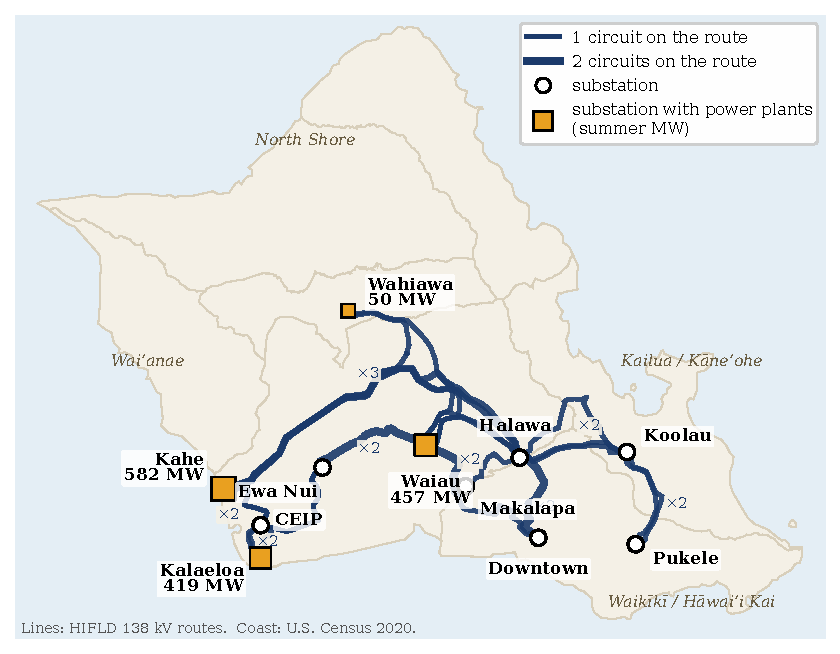
\includegraphics[width=\textwidth]{figs/fig1_map.pdf}
\caption{\textbf{\Oahu's 138\,kV transmission network as modelled.} Blue lines are the
real 138\,kV routes from the federal HIFLD map\src{HIFLD}; a thicker line carries two
circuits on one route, and ``$\times n$'' gives the number of circuits in a corridor.
Squares are substations with power plants attached, sized by their summer capacity
(EIA-860\src{EIA860}). The coastline is the Census 2020 shoreline\src{CB}.}
\label{fig:map}
\end{figure}

\Cref{fig:map} shows the network. It was assembled from four kinds of public record:
\begin{itemize}
  \item \textbf{Which substations exist and where:} the federal HIFLD map of
        transmission lines\src{HIFLD}. Each \SI{138}{kV} line in it names the two
        substations it joins; a substation sits where all of its lines meet.
  \item \textbf{How many circuits join each pair:} the utility's single-line diagrams
        in its 2021 Renewable Energy Zone study\src{REZ}, which name existing circuits
        one by one (``Kahe--Halawa \#1'', ``Waiau--Makalapa 2''); a worked example
        in its IGP interconnection appendix\src{RFP} (``Waiau-Ewa Nui 1 and Waiau-Ewa Nui
        2 138kV circuits'');
        and the Public Utilities Commission's 2007 order on the East \Oahu{}
        Transmission Project\src{PUC} (``Two 138kv transmission lines currently feed
        the Pukele Substation from the Koolau Substation'').
  \item \textbf{How long each line is:} measured along the HIFLD route itself.
  \item \textbf{Where each power plant connects:} its own switchyard (Kahe, Waiau), the
        nearest \SI{138}{kV} substation (Schofield at Wahiaw\=a), or --- for H-Power,
        Kalaeloa and CIP CT-1 --- the AES switching station, whose line the utility
        describes as carrying power ``from existing independent power producers AES,
        H-Power, and Kalaeloa, as well as from Hawaiian Electric's CIP CT-1 generating
        unit''\src{AES}.
\end{itemize}

Three simplifications are made. The downtown substations --- Iwilei and School Street,
which the Commission names as the two serving downtown, and Archer, Kewalo and Kamoku,
which it also mentions\src{PUC} --- are merged into one bus, \emph{Downtown}: HIFLD draws
only one of them (Kewalo), and no public source shows how they are wired to each other.
The three circuits that feed downtown from outside --- ``three 138kv transmission lines
providing power from the Halawa and Makalapa Substations''\src{PUC} --- are kept. The
AES switching station and the Kalaeloa plant, \SI{0.46}{mi} apart on the HIFLD map, are
merged into one bus, \emph{Kalaeloa}. And the
\SI{46}{kV} sub-transmission network below the \SI{138}{kV} system is not modelled
(\cref{sec:limits}).

\begin{table}[!htbp]
\centering
\small
\caption{\textbf{The 16 corridors.} Rating is per corridor (circuits $\times$
\SI{209.9}{MW}). Circuit counts: \src{REZ}, \src{RFP}, \src{AES} and \src{PUC} as
listed; otherwise the number of HIFLD routes.}
\label{tab:lines}
\begin{tabular}{@{}lrrrl@{}}
\toprule
\textbf{Corridor} & \textbf{Circuits} & \textbf{Miles} & \textbf{Rating (MW)} &
  \textbf{Circuit count from} \\
\midrule
Kahe--CEIP           & 2 & 4.26  & 419.7 & HIFLD; \src{AES} (``Kahe-CEIP 1\&2'') \\
CEIP--Kalaeloa       & 2 & 2.15  & 419.7 & HIFLD (two routes); \src{AES} \\
Kalaeloa--Ewa Nui    & 1 & 8.29  & 209.9 & HIFLD \\
CEIP--Ewa Nui        & 1 & 6.58  & 209.9 & HIFLD \\
Ewa Nui--Waiau       & 2 & 7.21  & 419.7 & \src{REZ} Fig.~34; \src{RFP} \\
Kahe--Waiau          & 1 & 18.81 & 209.9 & HIFLD \\
Kahe--Halawa         & 3 & 20.69 & 629.6 & \src{REZ} Figs.~30, 33 (with Kahe--Makalapa) \\
Kahe--Wahiawa        & 1 & 17.82 & 209.9 & HIFLD; \src{REZ} Fig.~32 (Akau--Wahiawa) \\
Wahiawa--Waiau       & 1 & 12.23 & 209.9 & \src{REZ} Fig.~32, Table~5-3 \\
Waiau--Makalapa      & 2 & 4.52  & 419.7 & \src{REZ} Fig.~34 \\
Waiau--Koolau        & 2 & 13.28 & 419.7 & \src{REZ} Table 10-3 (\#1, \#2); \src{PUC} \\
Halawa--Koolau       & 1 & 9.71  & 209.9 & \src{REZ} Figs.~30, 31; \src{PUC} \\
Halawa--Makalapa     & 1 & 4.26  & 209.9 & HIFLD \\
Halawa--Downtown     & 2 & 6.26  & 419.7 & \src{REZ} Fig.~30 (Iwilei, School St) \\
Makalapa--Downtown   & 1 & 7.09  & 209.9 & \src{PUC} (third downtown circuit) \\
Koolau--Pukele       & 2 & 6.32  & 419.7 & \src{PUC}; \src{REZ} Fig.~31 \\
\midrule
\textbf{Total} & \textbf{25} & & & \\
\bottomrule
\end{tabular}
\end{table}

\paragraph{Two numbers are stand-ins.} The utility does not publish the reactance or
the rating of its existing lines, so both come from the closest documented source.
\begin{itemize}
  \item \textbf{Rating: \SI{209.9}{MW} per circuit.} In its 2021 study the utility draws
        the new \SI{138}{kV} circuits it would build into Halawa as single ``795 AAC''
        conductors (Figs.~30, 33, 36), and when it re-conductors existing lines it
        specifies ``double-bundled 795 AAC'' (Table 5-3)\src{REZ} --- so the existing
        lines it would upgrade carry less than two such conductors today. We use one
        \SI{795}{kcmil} all-aluminium conductor per circuit. Its manufacturer rates it
        at \SI{878}{A}\src{SW} (\SI{75}{\celsius} conductor, \SI{25}{\celsius} air,
        \SI{2}{ft/s} wind, in sun), and one three-phase circuit then carries
        $\sqrt{3}\times\SI{138}{kV}\times\SI{878}{A} = \SI{209.9}{MVA}$. Picture the rating
        as the width of the pipe: a thicker wire carries more current before it heats
        up and sags. For one corridor this is probably low: the utility's 2016
        application to move part of the AES--CEIP 2 circuit specifies a
        \SI{1780}{kcmil} conductor for the new section\src{AES}. Because the true
        ratings are unknown, every result is repeated with \SI{150}{MW} per circuit
        (three times the surge impedance loading of a typical \SI{138}{kV} line, the
        usual limit for short lines\src{UT}) and with \SI{318.6}{MW} (the
        \SI{1590}{kcmil} conductor the utility labels on its planned new Kahe--Wahiawa
        and Makalapa circuits\src{REZ}, rated \SI{1333}{A}\src{SW}; the same study's
        tables print ``1950 AAC'' for some of these circuits, which is not a standard
        size); see \cref{sec:sens}.
  \item \textbf{Reactance: \SI{0.48}{\ohm/km}}, the typical value for a
        \SI{138}{kV} line with one conductor per phase\src{UT}, the same quantity synthetic-grid
        builders compute from conductor geometry\src{GEG}. Because every line gets the
        same ohms per mile, this number \emph{cancels out}: power divides between
        parallel paths in proportion to $1/\text{length}$ whatever the ohms per mile.
        Only the lengths, which are measured, matter.
\end{itemize}

\subsection{The generators}

The fleet is the island's 24 dispatchable units as reported to the U.S. Energy
Information Administration for 2024\src{EIA860}, \SI{1508.1}{MW} in total. Each unit's
running cost is its measured heat rate\src{EIA923} times the utility's 2024 fuel-price
forecast\src{IGP}, plus a variable maintenance cost. That cost is a stand-in: the
utility publishes values only for \emph{new} combined-cycle, combustion-turbine and
engine plants\src{IGP}, which we use for its existing ones, and none at all for steam
or waste-to-energy units, for which we use the U.S.\ EPA's values for existing
units\src{EPA}. It is small next to fuel and changes no unit's place in the order in
which plants are run. H-Power burns the island's municipal waste and is given no fuel
cost, which makes it the first plant to run.

\begin{center}
\small
\begin{tabular}{@{}llrr@{}}
\toprule
\textbf{Plant} & \textbf{Substation} & \textbf{MW} & \textbf{\$/MWh} \\
\midrule
H-Power (waste-to-energy)      & Kalaeloa & 86.0  & 6.94 \\
Kalaeloa (combined cycle)      & Kalaeloa & 220.0 & 94.05 \\
Kahe 1--6 (oil steam)          & Kahe     & 582.1 & 122.28 \\
Waiau 3--8 (oil steam)         & Waiau    & 354.2 & 130.36 \\
Schofield (engines)            & Wahiawa  & 50.4  & 173.33 \\
Waiau 9--10 (combustion turbines) & Waiau & 102.4 & 224.84 \\
CIP CT-1 (combustion turbine)  & Kalaeloa & 113.0 & 240.47 \\
\midrule
\textbf{Total} & & \textbf{1508.1} & \\
\bottomrule
\end{tabular}
\end{center}

Utility-scale solar, wind and batteries are not in this fleet; the demand the fleet
must meet is the island load net of rooftop solar (\cref{sec:stats}). The fleet
therefore has to cover the whole net load by itself, which makes the model
conservative about supply.

%======================================================================
\section{How the substation statistics are obtained}
\label{sec:stats}
%======================================================================

\subsection{Demand at each substation, hour by hour}

The model needs $d_n$ for every substation in every hour. No public record gives it,
so it is built in three steps from records that do exist.

\begin{enumerate}
  \item \textbf{The island total.} The utility's filed hourly load for 2021
        (Integrated Grid Planning inputs, Workbook~3\src{IGP}), \num{8760} values.
        It is the load the grid must deliver: customer demand minus rooftop solar,
        customer batteries and energy efficiency, each an hourly layer in the same
        workbook. This total is kept exactly.
  \item \textbf{Who is where.} Every 2020 census tract (people\src{CEN}) and every
        census block with jobs (LEHD LODES 2021\src{LODES}) is given to its nearest
        load-serving \SI{138}{kV} substation --- each substation serves its own
        ``catchment'', the rule the open European grid model PyPSA-Eur uses for the same
        purpose\src{PYPSA}. The Ko\okina olau mountains are respected: a neighbourhood is served only from
        a substation on its own side of the range (the thinly populated north-east
        shore, Ko\okina olauloa, may also be served around the north end, from
        Wahiaw\=a). The utility's
        list of the neighbourhoods fed from Pukele (``Kahala, Kaimuki, Manoa, Makiki,
        and Waikiki''\src{PUC}) is followed and extended east to Hawai\okina i Kai:
        census tracts 1--35, which run from Hawai\okina i Kai west to Makiki, and any
        tract east of \ang{157.830}\,W go to Pukele.
  \item \textbf{What kind of load, hour by hour.} The island's sales are split into
        homes, businesses and industry by the utility's 2021 sales\src{EIA861}; each
        sector gets its own daily shape (U.S.\ DOE reference buildings for
        Honolulu\src{OEI}; flat for industry). Homes follow people and businesses follow
        jobs. Rooftop solar and efficiency are subtracted where their own sector
        shares\src{EIA861} say they are.
\end{enumerate}

\paragraph{The same three steps as one equation.} Picture three buckets of paint ---
homes, businesses, industry. Every hour each bucket holds a different amount: the
island's load in that sector. Every substation pours from the same three buckets with
its own \emph{fixed recipe}. For substation $b$ in hour $t$:
\begin{equation}
  d_b(t) \;=\; k_{b,\text{res}}\,N_{\text{res}}(t) \;+\; k_{b,\text{com}}\,N_{\text{com}}(t)
  \;+\; k_{b,\text{ind}}\,N_{\text{ind}}(t),
  \label{eq:demand}
\end{equation}
or, for all ten substations with load at once,
\[
  \underbrace{D}_{10\times 8760} \;=\; \underbrace{K}_{10\times 3}\;
  \underbrace{N}_{3\times 8760}.
\]

\begin{center}
\small
\begin{tabular}{@{}lp{0.36\textwidth}p{0.4\textwidth}@{}}
\toprule
\textbf{Symbol} & \textbf{Material object} & \textbf{Where it comes from} \\
\midrule
$N_s(t)$ & how full \textbf{bucket} $s$ is in hour $t$: the island's load of sector $s$,
  in MW & the filed island total, split by 2021 sales shares\src{EIA861} and hourly
  shapes\src{OEI}, minus that sector's share of rooftop solar, efficiency and
  batteries \\
$k_{b,s}$ & substation $b$'s \textbf{recipe}: its share of the island's people (homes),
  commercial jobs (businesses) or industrial jobs (industry) & census 2020\src{CEN} and
  LODES 2021\src{LODES}; the same in every hour \\
$d_b(t)$ & what substation $b$ pours in hour $t$, in MW & the product \\
\bottomrule
\end{tabular}
\end{center}

\noindent Over 2021 the three buckets average \SI{147}{MW} (homes; below zero at sunny
middays, when rooftop solar exceeds home use), \SI{215}{MW} (businesses) and
\SI{382}{MW} (industry). The recipes are:

\begin{center}
\small
\begin{tabular}{@{}lrrr@{\hspace{2.2em}}lrrr@{}}
\toprule
& \multicolumn{3}{c}{\textbf{share of island (\%)}} & & \multicolumn{3}{c}{\textbf{share of island (\%)}} \\
\textbf{Substation} & people & com.\ jobs & ind.\ jobs & \textbf{Substation} & people & com.\ jobs & ind.\ jobs \\
\midrule
Downtown & 13.0 & 46.2 & 41.6 & Ewa Nui & 12.7 & 3.6 & 5.9 \\
Pukele   & 21.6 & 19.6 & 6.2  & Wahiawa & 12.4 & 4.6 & 5.3 \\
Makalapa & 6.0  & 9.3  & 14.1 & Koolau  & 11.9 & 5.3 & 4.7 \\
CEIP     & 4.1  & 3.1  & 12.2 & Kahe    & 5.6  & 1.7 & 1.2 \\
Waiau    & 9.6  & 6.0  & 8.0  & Halawa  & 3.2  & 0.7 & 0.7 \\
\bottomrule
\end{tabular}
\end{center}

The result is an $11 \times \num{8760}$ table of megawatts (Kalaeloa, a switching
station, has no load). Its one public check is three substation shares the utility gave the Commission in
2007\src{PUC}: Pukele ``supplied electricity to approximately seventeen percent of the
Oahu load'' at the 2002 day peak (our table: \SI{14.1}{\percent} at the 2021 day peak);
Koolau and Pukele together serve ``approximately thirty percent'' (no date given; ours:
\SI{20.3}{\percent}); and Iwilei, School Street and the Honolulu Power Plant served
``about twenty-five percent'' at the 2002 day peak (ours: \SI{38.4}{\percent}, for a
Downtown bus that also holds Archer, Kewalo and Kamoku, Kaka\okina ako and Ala Moana).
The filed shares are nineteen years older and partly cover different substations, so
they are not a target; but because they differ, every result is repeated with the
table re-weighted to match them (\cref{sec:sens}).

\subsection{The Gaussian model of each substation}

Each substation now has \num{8760} numbers. We summarise them with a
\textbf{Gaussian (normal) distribution}, the bell curve:
\[
  d_n \;\sim\; \mathcal{N}\!\left(\mu_n,\ \sigma_n^{2}\right),
  \qquad
  f(x) = \frac{1}{\sigma_n\sqrt{2\pi}}\;
         \exp\!\left(-\frac{(x-\mu_n)^2}{2\sigma_n^2}\right),
\]
\[
  \mu_n = \frac{1}{8760}\sum_{h=1}^{8760} d_{n,h},
  \qquad
  \sigma_n^{2} = \frac{1}{8759}\sum_{h=1}^{8760}\left(d_{n,h} - \mu_n\right)^{2}.
\]
Picture a sandpile. Pour one grain for each hour of the year onto a ruler marked in
megawatts, at the demand that hour had. $\mu_n$ is where the pile balances; $\sigma_n$
is how wide it spreads --- about two thirds of the grains of a true bell-shaped pile lie
within one $\sigma_n$ of the middle.

\begin{table}[!htbp]
\centering
\small
\caption{\textbf{The Gaussian of each substation.} $\mu$ and $\sigma$ from the
\num{8760} hours of 2021. $\sigma/\mu$ strips out size and leaves only how much a
substation swings. Share: share of the island at the 2021 day peak (the 50 heaviest
hours between 10:00 and 16:00).}
\label{tab:gauss}
\begin{tabular}{@{}llrrrr@{}}
\toprule
\textbf{Substation} & \textbf{Serves} & \textbf{$\mu$ (MW)} & \textbf{$\sigma$ (MW)} &
  \textbf{$\sigma/\mu$} & \textbf{Share} \\
\midrule
Downtown & downtown, Kalihi, Kaka\okina ako, Ala Moana & 277.2 & 35.3 & 0.13 & 38.4\% \\
Pukele   & Waik\=ik\=i, M\=anoa, Kaimuk\=i, K\=ahala, Hawai\okina i Kai & 97.6 & 26.6 & 0.27 & 14.1\% \\
Makalapa & Pearl Harbor, Hickam, Salt Lake & 82.5 & 9.1 & 0.11 & 10.8\% \\
CEIP     & Campbell Industrial Park, Kapolei & 59.5 & 5.3 & 0.09 & 7.3\% \\
Waiau    & Pearl City, Waipahu, Mililani & 57.4 & 10.8 & 0.19 & 7.5\% \\
Ewa Nui  & \=Ewa, \=Ewa Beach & 48.9 & 13.6 & 0.28 & 6.2\% \\
Wahiawa  & Wahiaw\=a, Schofield, the North Shore & 48.2 & 13.4 & 0.28 & 6.2\% \\
Koolau   & K\=ane\okina ohe, Kailua, the windward coast & 47.0 & 13.1 & 0.28 & 6.2\% \\
Kahe     & the Wai\okina anae coast & 16.6 & 6.0 & 0.36 & 2.2\% \\
Halawa   & \okina Aiea, H\=alawa & 8.8 & 3.4 & 0.39 & 1.1\% \\
Kalaeloa & --- (switching station) & 0 & 0 & --- & --- \\
\midrule
\textbf{Island} & & \textbf{743.9} & \textbf{124.9} & \textbf{0.17} & \\
\bottomrule
\end{tabular}
\end{table}

\begin{figure}[!htbp]
\centering
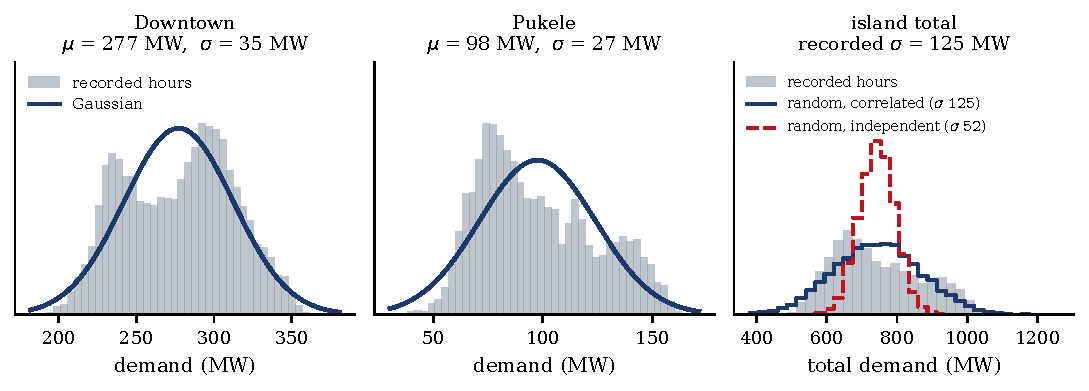
\includegraphics[width=\textwidth]{figs/fig2_gaussian.pdf}
\caption{\textbf{The bell curves behind the random draws.} \emph{Left and centre:}
grey bars are the \num{8760} recorded hours at two substations; the blue curve is the
Gaussian drawn from only the $\mu$ and $\sigma$ above each panel. The curve gets the
centre and the spread right but not the shape: real demand has two humps, a night hump
and a day hump. \emph{Right:} the island total. Correlated draws (blue) have the same
spread as the recorded year; independent draws (red dashes) have well under half of it.}
\label{fig:gauss}
\end{figure}

\Cref{fig:gauss} is honest about the fit. The bell has the right middle and the right
width, but the recorded hours are two-humped: \SI{61}{\percent} of Downtown's hours and
\SI{65}{\percent} of Pukele's lie within one $\sigma$ of the mean, against
\SI{68}{\percent} for a true bell. The Gaussian is a summary, not a copy.

\subsection{The substations move together}

Drawing each substation from its own bell curve \emph{separately} gives eleven correct
substations and a wrong island. The island total is a sum, and a sum of independent
terms cancels most of their swings. Real substations do not cancel: when \Oahu{} is busy
it is busy everywhere at once. Over the recorded year every pair of substations is
positively correlated (from \num{0.47} to \num{1.00}, average \num{0.86}).

\begin{center}
\small
\begin{tabular}{@{}lrrrr@{}}
\toprule
\textbf{Demand input} & \textbf{Mean} & \textbf{Std.\ dev.} & \textbf{Highest} &
  \textbf{Hours above \SI{1000}{MW}} \\
\midrule
the recorded year (\num{8760} hours)            & \SI{743.9}{MW} & \SI{124.9}{MW} & \SI{1054.3}{MW} & \SI{1.83}{\percent} \\
eleven bells drawn \emph{separately} (\num{10000}) & \SI{743.6}{MW} & \SI{52.0}{MW}  & \SI{960.2}{MW}  & \SI{0.00}{\percent} \\
eleven bells drawn \emph{together} (\num{10000})   & \SI{743.0}{MW} & \SI{125.1}{MW} & \SI{1216.0}{MW} & \SI{1.89}{\percent} \\
\bottomrule
\end{tabular}
\end{center}

So the random draws use the \textbf{multivariate Gaussian}: the same eleven means,
plus the measured $11\times 11$ covariance matrix $\Sigma$, which records how every
pair of substations moves together:
\[
  \mathbf{d} \;=\; \max\!\left(\mathbf{0},\ \boldsymbol{\mu} + L\,\mathbf{z}\right),
  \qquad \mathbf{z} \sim \mathcal{N}(\mathbf{0},\, I_{11}),
  \qquad L L^{\top} = \Sigma .
\]
Picture eleven corks on one pond. $\mathbf{z}$ is a handful of random waves; $L$ is
the shape of the pond, which decides how each wave lifts every cork at once. Each cork
still bobs exactly as much as its own $\sigma_n$ says, but now they rise and fall
together as the real substations do. The draw is floored at zero because demand cannot
be negative.

\paragraph{Why $\Sigma$ is singular, and what we do about it.} Because $D = KN$,
every substation's demand is a mix of the same three bucket
curves, so the ten substations with load have only three independent directions of
change: $\Sigma = K\,\Sigma_N K^{\top}$ has rank three, with eigenvalues
\num{2295}, \num{452} and \SI{17}{MW^2} and seven exact zeros. Two things follow.
Any substation is an exact mix of three others: Pukele $= 0.338\,$Downtown
$+\,1.875\,$Wahiaw\=a $-\,1.456\,$CEIP in every hour, to within \SI{0.0002}{MW}. And two
substations with nearly the same recipe are nearly proportional: Koolau stays between
0.95 and 1.00 times Wahiaw\=a all year (correlation 0.999).

Real substations do not behave like this. Each also moves on its own --- local weather
and clouds over rooftop solar, one hospital or base changing its load, switching ---
so metered data would give a full-rank, if highly correlated, $\Sigma$. The singularity
is a property of how our demand table is built, not of \Oahu. It has a technical
consequence: $L$ comes from an eigendecomposition of $\Sigma$, because the usual
Cholesky factorisation fails on a singular matrix. It also has a substantive one: the
draws can never produce one substation rising on its own. So every outage test is
repeated with a \textbf{local wiggle} added to each substation (\cref{sec:noise}):
\begin{equation}
  \mathbf{d} \;=\; \max\!\left(\mathbf{0},\ \boldsymbol{\mu} + L\,\mathbf{z}
  + f\,\boldsymbol{\sigma}\odot\boldsymbol{\eta}\right),
  \qquad \boldsymbol{\eta} \sim \mathcal{N}(\mathbf{0}, I),
  \qquad \operatorname{Cov}(\mathbf{d}) \approx \Sigma + f^2\operatorname{diag}(\sigma_n^2).
  \label{eq:noise}
\end{equation}
The waves $\mathbf{z}$ still lift every cork together; $\boldsymbol{\eta}$ gives each cork
its own small independent bob, $f$ times its usual swing $\sigma_n$. The added
diagonal makes the covariance full rank. The same wiggle is added to the recorded
hours.

One consequence matters for the results. The Gaussian's tails are longer than the
recorded year's: the random draws reach \SI{1216}{MW}, \SI{15}{\percent} above the
recorded peak of \SI{1054}{MW}, and \SI{0.56}{\percent} of draws exceed that peak. The
random input is therefore a stress test of the year, not a replay of it.

%======================================================================
\section{The experiments}
\label{sec:exp}
%======================================================================

The same linear program is solved again and again. Between solves only two things
change: the demand vector $\mathbf{d}$, and which lines are in service.

\begin{center}
\small
\begin{tabular}{@{}lp{0.62\textwidth}@{}}
\toprule
\textbf{Demand input} & \\
\midrule
\textbf{recorded} & the \num{8760} hourly demand vectors of 2021, one solve per hour \\
\textbf{random}   & \num{10000} vectors drawn from the multivariate Gaussian of
                    \cref{sec:stats}, one solve per draw \\
\midrule
\textbf{Network state} & \\
\midrule
\textbf{N-0} & every circuit in service (1 case) \\
\textbf{N-1} & one circuit out, each in turn (16 distinct cases: the circuits of a
               corridor are identical, so losing either of two is the same case) \\
\textbf{N-2} & two circuits out, every pair (128 distinct cases). This is the
               utility's own planning test: ``no transmission component shall exceed its
               emergency rating with one generating unit on overhaul, one transmission
               line out for maintenance and loss of a second transmission
               line''\src{PUC} \\
\textbf{growth} & every line in service, every demand multiplied by
               $g = 1.0, 1.1, \dots, 2.0$ \\
\midrule
\textbf{Local variation} & \\
\midrule
$f = 0.10, 0.25, 0.50$ & N-0, N-1, N-2 and growth repeated with each substation's own
               wiggle added (\cref{eq:noise}), in every recorded hour and random draw \\
\bottomrule
\end{tabular}
\end{center}

Each outage case is solved on all \num{8760} recorded hours \emph{and} all \num{10000}
random draws, so every percentage below is a share of \emph{all} hours or \emph{all}
draws, not of a sample. Two remarks on the outage test. It uses normal ratings, because
emergency ratings are not published; since a real line may run above its normal rating
for a few hours after a second failure, our N-2 results are the conservative
(pessimistic) side of the utility's test. And the generators are allowed to
re-dispatch after the outage, as they would be.

%======================================================================
\section{Results}
\label{sec:results}
%======================================================================

\subsection{All lines in service: nothing goes wrong}

\begin{figure}[!htbp]
\centering
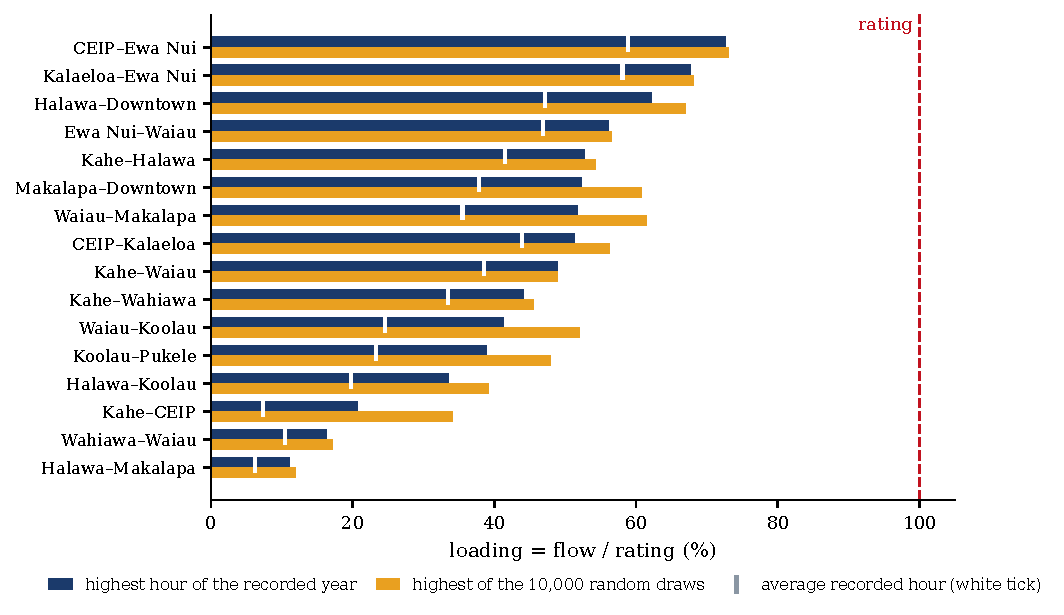
\includegraphics[width=0.9\textwidth]{figs/fig3_normal.pdf}
\caption{\textbf{How full each line gets with every line in service.} Loading is flow
divided by rating. Blue: the heaviest hour of the recorded year; gold: the heaviest of
the \num{10000} random draws; white tick: the average recorded hour. No line reaches
its rating (red dashes) in any hour or any draw.}
\label{fig:normal}
\end{figure}

With every circuit in service, \textbf{all demand is served in all \num{8760} recorded
hours and all \num{10000} random draws, and no line ever reaches its rating}
(\cref{fig:normal}). The fullest line is CEIP--Ewa Nui, at \SI{72.6}{\percent} in its
heaviest recorded hour and \SI{73.0}{\percent} in the heaviest random draw; the next are
Kalaeloa--Ewa Nui (\SI{68}{\percent}) and Halawa--Downtown (\SI{62}{\percent} recorded,
\SI{67}{\percent} random). This is consistent with the utility's own 2021 power-flow study,
which found ``no existing system equipment overloading issue'' in the conditions it
studied\src{REZ}.

The two fullest lines have the same job: they carry the west side's power \emph{east}
--- all of the output of the island's two cheapest plants, H-Power and the Kalaeloa
combined cycle (\SI{306}{MW} between them, run in every hour), plus part of Kahe's.
Everything generated west of Ewa Nui except what goes north on the Kahe lines has to
cross one of these two single circuits.

The random draws load the lines a little more than the recorded year (for
Waiau--Makalapa, \SI{61}{\percent} against \SI{52}{\percent}) because their tails reach
higher demand, but they never reach a rating either.

\subsection{One circuit lost (N-1): no demand lost, two lines pinned}

Removing any one of the 25 circuits, in any recorded hour or any random draw,
\textbf{never leaves demand unserved}. What changes is that some lines are pushed to
their rating, and the optimiser has to re-dispatch --- run dearer plant elsewhere ---
to keep them there:

\begin{center}
\small
\begin{tabular}{@{}llrr@{}}
\toprule
\textbf{Circuit lost} & \textbf{Line pushed to its rating} &
  \textbf{Recorded hours} & \textbf{Random draws} \\
\midrule
Kalaeloa--Ewa Nui          & CEIP--Ewa Nui      & \num{3401} (\SI{38.8}{\percent}) & \num{4235} (\SI{42.4}{\percent}) \\
CEIP--Ewa Nui              & Kalaeloa--Ewa Nui  & \num{2359} (\SI{26.9}{\percent}) & \num{2523} (\SI{25.2}{\percent}) \\
one Halawa--Downtown circuit & the other one    & 1 (\SI{0.01}{\percent})          & 32 (\SI{0.32}{\percent}) \\
one CEIP--Kalaeloa circuit & the other one      & 0                                & 17 (\SI{0.17}{\percent}) \\
one Waiau--Makalapa circuit & the other one     & 0                                & 4 (\SI{0.04}{\percent}) \\
\bottomrule
\end{tabular}
\end{center}

\noindent The first two rows are the export pair again. Lose one of the two single
circuits east of Kalaeloa and the other is full for a quarter to two fifths of the year.
The optimiser does not touch the cheap Kalaeloa plants (they stay at \SI{306}{MW});
it runs Kahe less --- Kahe's power also reaches the full line, through CEIP --- and
Waiau, which is east of the bottleneck, more. With Kalaeloa--Ewa Nui out, Kahe gives up
\SI{61}{MW} on average in the pinned hours and Waiau adds the same, at an extra running
cost of \$491 per pinned hour. The system still meets the utility's single-outage
test, but the margin that makes it pass is \emph{generation that can be moved}, not
spare wire.

\subsection{Two circuits lost (N-2): four areas can lose power}

Of the 128 ways to lose two circuits, \textbf{7 leave demand unserved in the recorded
year, and 10 in the random draws} (\cref{tab:n2,fig:n2}). In the recorded year they
fall into four areas, and each has one simple reason: it hangs off two or three
circuits, and two failures leave it with too little wire, or none. The random draws
add a fifth, rarely: Pearl Harbor (Makalapa).

\begin{table}[!htbp]
\centering
\small
\caption{\textbf{The double outages that leave demand unserved.} Hours: share of the
\num{8760} recorded hours with any unserved demand; draws: share of the \num{10000}
random draws. MWh: total unserved over the recorded year. Worst: the largest unserved
demand in any single recorded hour. ``One X circuit'' means one of the parallel circuits
of corridor X.}
\label{tab:n2}
\begin{tabular}{@{}p{0.3\textwidth}p{0.2\textwidth}rrrr@{}}
\toprule
\textbf{Circuits lost} & \textbf{Area short} & \textbf{Hours} & \textbf{Draws} &
  \textbf{MWh / yr} & \textbf{Worst} \\
\midrule
both Koolau--Pukele circuits & East Honolulu & 100\% & 99.99\% & \num{854579} & \SI{163}{MW} \\
both Halawa--Downtown circuits & Downtown & 98.9\% & 97.4\% & \num{590276} & \SI{160}{MW} \\
one Halawa--Downtown circuit + Makalapa--Downtown & Downtown & 98.9\% & 97.4\% & \num{590709} & \SI{160}{MW} \\
Kahe--Wahiawa + Wahiawa--Waiau & Wahiaw\=a, North Shore & 36.8\% & 43.1\% & \num{41750} & \SI{29}{MW} \\
both Waiau--Koolau circuits & Windward + East Honolulu & 7.9\% & 4.9\% & \num{6893} & \SI{31}{MW} \\
one Waiau--Koolau circuit + Halawa--Koolau & Windward + East Honolulu & 7.9\% & 4.9\% & \num{6927} & \SI{31}{MW} \\
one Waiau--Makalapa + one Halawa--Downtown circuit & Downtown & 0.01\% & 0.53\% & 5 & \SI{5}{MW} \\
\midrule
\multicolumn{6}{@{}l}{\textit{Only in the random draws}}\\
one Kahe--Halawa + one Waiau--Makalapa circuit & Pearl Harbor (Makalapa) & 0 & 0.33\% & 0 & --- \\
one Waiau--Makalapa + one Waiau--Koolau circuit & Pearl Harbor (Makalapa) & 0 & 0.08\% & 0 & --- \\
Halawa--Koolau + one Halawa--Downtown circuit & Downtown & 0 & 0.01\% & 0 & --- \\
\bottomrule
\end{tabular}
\end{table}

\begin{figure}[!htbp]
\centering
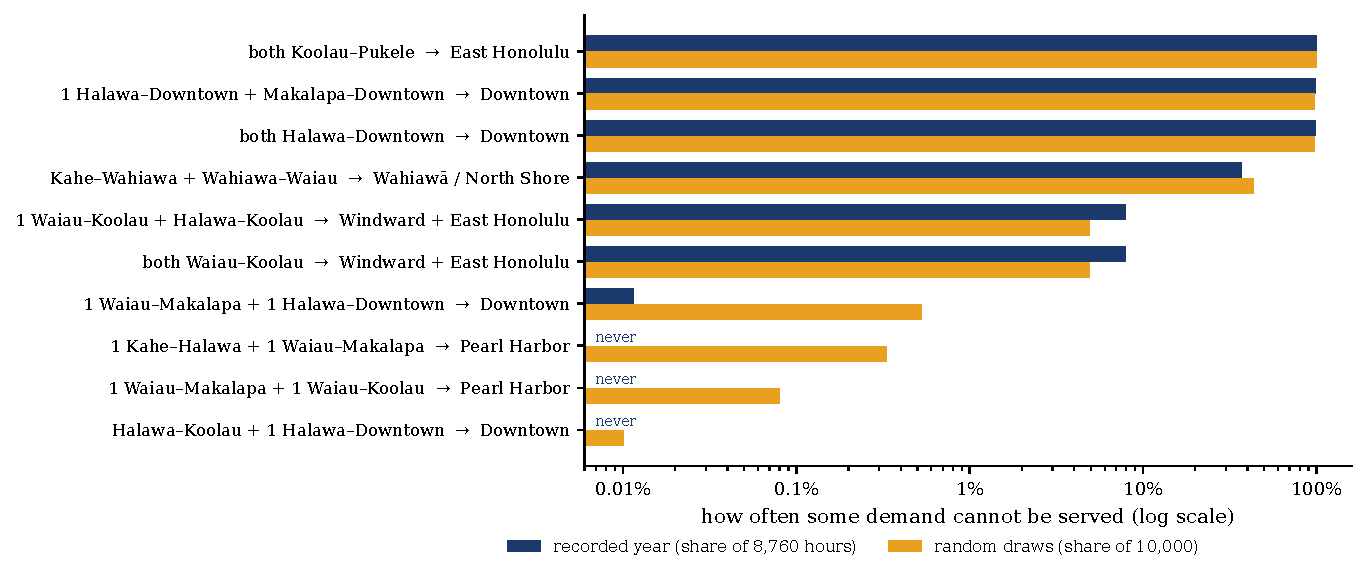
\includegraphics[width=\textwidth]{figs/fig4_outages.pdf}
\caption{\textbf{Two circuits lost: how often each area cannot be fully served.} Every
double outage that leaves demand unserved in either input; ``1 X'' means one of the
parallel circuits of corridor X, ``both X'' means both. Log scale: each gridline is ten
times the one before. Blue, the recorded year; gold, the random draws.}
\label{fig:n2}
\end{figure}

\begin{description}[leftmargin=1.2em,style=nextline]
  \item[East Honolulu (Pukele) --- the largest single exposure.] Pukele serves
        Waik\=ik\=i, M\=anoa, Kaimuk\=i, K\=ahala and Hawai\okina i Kai and is fed at
        \SI{138}{kV} by exactly two circuits, both from Koolau\src{PUC}. Lose both and
        there is no \SI{138}{kV} path at all: the whole Pukele load, up to
        \SI{163}{MW}, is unserved in every hour. The utility told the Commission the
        same: if both lines are out, ``approximately ninety-three percent of the
        customers serviced from the Pukele Substation will experience an
        outage''\src{PUC}. The 2007 order approved a \SI{46}{kV} project that ``will
        allow load to be shifted among the three substations using 46kv
        lines''\src{PUC} --- Pukele, Archer and Kamoku. That \SI{46}{kV} backstop is
        outside our model, so this row is what the \SI{138}{kV} network alone would do.
  \item[Downtown Honolulu --- the utility's own ``Downtown Overload Situation''.]
        Downtown is fed by three circuits (two from Halawa, one from Makalapa). Lose any
        two and the last one carries at most \SI{209.9}{MW}, while downtown's demand runs
        from \SI{192}{MW} to \SI{370}{MW} and is above \SI{209.9}{MW} in 8,661 of the
        \num{8760} hours --- exactly the hours in which demand goes unserved
        (\SI{99}{\percent}).
        The utility described the same event to the Commission: if one downtown line is
        out for maintenance ``and a second Downtown 138kv transmission line becomes
        unavailable, then the current flowing through the remaining Downtown 138kV
        transmission line will exceed the emergency current carrying capacity
        rating''\src{PUC}. It expected this from 2007 without the Honolulu Power Plant
        downtown\src{PUC}; that plant is no longer in the fleet\src{EIA860}.
  \item[Wahiaw\=a and the North Shore.] Wahiaw\=a has two \SI{138}{kV} lines, one to
        Kahe and one to Waiau\src{HIFLD} (the utility's diagram names them Akau--Wahiawa
        and Waiau--Wahiawa\src{REZ}). Lose both and it becomes an island with only the
        \SI{50.4}{MW} Schofield plant, which covers its demand in the lighter
        \SI{63}{\percent} of hours and falls short, by up to \SI{29}{MW}, in the other
        \SI{37}{\percent}.
  \item[The windward side and East Honolulu together.] Koolau (and Pukele behind it) is
        fed by three circuits\src{PUC}. Lose two and the third carries the whole
        windward-plus-East-Honolulu load alone; in the heaviest \SI{8}{\percent} of
        hours it cannot. The utility projected exactly this: with one Koolau line out for
        maintenance and a second unavailable, ``the current flowing through the third
        138kV Koolau transmission line will exceed its emergency current carrying
        capacity rating during daytime peak load conditions''\src{PUC}.
\end{description}

\paragraph{Real against random.} The two inputs agree on all seven recorded failures,
and within about six percentage points on how often they happen. Where they differ, the
random draws are reaching demands the recorded year never had: an island total above
the recorded peak, one substation above its own recorded maximum, or a mix of
substation demands the year never produced. That is why the random input finds three
extra rare cases (Pearl Harbor twice, downtown once), each in at most
\SI{0.33}{\percent} of draws and never in the recorded year, and why it makes the
downtown ``one Waiau--Makalapa + one Halawa--Downtown'' case about 46 times more
frequent (\SI{0.53}{\percent} of draws against one recorded hour,
\SI{0.011}{\percent}). For the windward rows the order flips (\SI{4.9}{\percent} of
draws against \SI{7.9}{\percent} of hours). Those failures happen whenever Koolau and
Pukele together need more than the \SI{210}{MW} one circuit can carry, and the real
year's upper hump puts more hours just above that line (\SI{7.87}{\percent}) than the
bell curve does (\SI{4.87}{\percent}): the Gaussian has the longer tail, the real year
the fatter shoulder.

\paragraph{Against the utility's own study.} The utility's 2021 power-flow study
checked normal, single-outage and double-outage conditions (the last at emergency
ratings) for the dispatches it studied and found ``no existing system equipment
overloading issue''\src{REZ}. Our model finds demand lost after some double outages.
The difference is what the model leaves out: emergency ratings, the real line ratings,
and the \SI{46}{kV} network that can move load between substations. So the rows of
\cref{tab:n2} show \emph{where the \SI{138}{kV} network is thinnest}; they are not a
prediction that customers there would lose power for that long.

\subsection{Which lines overload the most}

\Cref{tab:rank} ranks every line by how often it is pushed to its rating across all
outage cases. Read a cell ``$c$ / $h$'' as: in $c$ of the outage cases this line
reached its rating, for $h$ hours (or draws) in total across those cases.

\begin{table}[!htbp]
\centering
\small
\caption{\textbf{Every line, ranked by how often it reaches its rating.} N-0: highest
loading with every line in service. N-1 and N-2: number of outage cases in which the
line reaches its rating / total hours (recorded) or draws (random) at the rating,
summed over those cases. ``---'': never.}
\label{tab:rank}
\begin{tabular}{@{}lrrcccc@{}}
\toprule
& \multicolumn{2}{c}{\textbf{N-0 highest}} & \multicolumn{2}{c}{\textbf{N-1 (16 cases)}} &
  \multicolumn{2}{c}{\textbf{N-2 (128 cases)}} \\
\cmidrule(lr){2-3}\cmidrule(lr){4-5}\cmidrule(l){6-7}
\textbf{Line} & rec. & rand. & rec. & rand. & rec. & rand. \\
\midrule
CEIP--Ewa Nui & 73\% & 73\% & 1 / \num{3401} & 1 / \num{4235} & 14 / \num{50548} & 14 / \num{62724} \\
Kalaeloa--Ewa Nui & 68\% & 68\% & 1 / \num{2359} & 1 / \num{2523} & 14 / \num{48068} & 14 / \num{56284} \\
Halawa--Downtown & 62\% & 67\% & 1 / \num{1} & 1 / \num{32} & 13 / \num{9061} & 15 / \num{11113} \\
CEIP--Kalaeloa & 51\% & 56\% & --- & 1 / \num{17} & 2 / \num{8767} & 14 / \num{10371} \\
Makalapa--Downtown & 52\% & 61\% & --- & --- & 1 / \num{8663} & 1 / \num{9743} \\
Ewa Nui--Waiau & 56\% & 57\% & --- & --- & 3 / \num{4002} & 3 / \num{4955} \\
Waiau--Koolau & 41\% & 52\% & --- & --- & 1 / \num{702} & 1 / \num{503} \\
Halawa--Koolau & 34\% & 39\% & --- & --- & 1 / \num{698} & 1 / \num{501} \\
Waiau--Makalapa & 52\% & 61\% & --- & 1 / \num{4} & 3 / \num{83} & 8 / \num{295} \\
Kahe--Halawa & 53\% & 54\% & --- & --- & --- & --- \\
Kahe--Waiau & 49\% & 49\% & --- & --- & --- & --- \\
Kahe--Wahiawa & 44\% & 45\% & --- & --- & --- & --- \\
Koolau--Pukele & 39\% & 48\% & --- & --- & --- & --- \\
Kahe--CEIP & 21\% & 34\% & --- & --- & --- & --- \\
Wahiawa--Waiau & 16\% & 17\% & --- & --- & --- & --- \\
Halawa--Makalapa & 11\% & 12\% & --- & --- & --- & --- \\
\bottomrule
\end{tabular}
\end{table}

Three groups stand out.
\begin{itemize}
  \item \textbf{The export pair --- CEIP--Ewa Nui and Kalaeloa--Ewa Nui --- overloads
        the most}, by a wide margin: they are the two fullest lines in normal
        operation, the only lines pushed to their rating by a single outage in a large
        share of hours, and each is pushed to it in 14 of the 128 double outages. The
        cause is where the plants are --- the cheapest power on the island enters at
        Kalaeloa and must leave by these two single circuits --- and the heavier the
        island's load, the more often they fill: after a single outage the remaining
        one is full in every hour when the island needs more than
        \SI{833}{MW}, and in none below \SI{756}{MW}.
  \item \textbf{The three downtown feeders} --- two circuits from Halawa and one
        from Makalapa --- matter most for customers. Halawa--Downtown reaches its
        rating in 13 double outages. When a downtown feeder fills, the only relief is
        the other downtown feeders, because downtown has no plant of its own; that is
        why these are the overloads that end in lost demand. Under
        growth, Makalapa--Downtown and Waiau--Makalapa are the first lines to fill.
  \item \textbf{Seven lines never reach their rating in any case}: Kahe--Halawa,
        Kahe--Waiau, Kahe--Wahiawa, Koolau--Pukele, Kahe--CEIP, Wahiawa--Waiau and
        Halawa--Makalapa. Koolau--Pukele is on this list even though losing it is the
        worst outage on the island: it never overloads, it simply disappears.
\end{itemize}

\subsection{Demand growth: the generators run out before the wires}

\begin{figure}[!htbp]
\centering
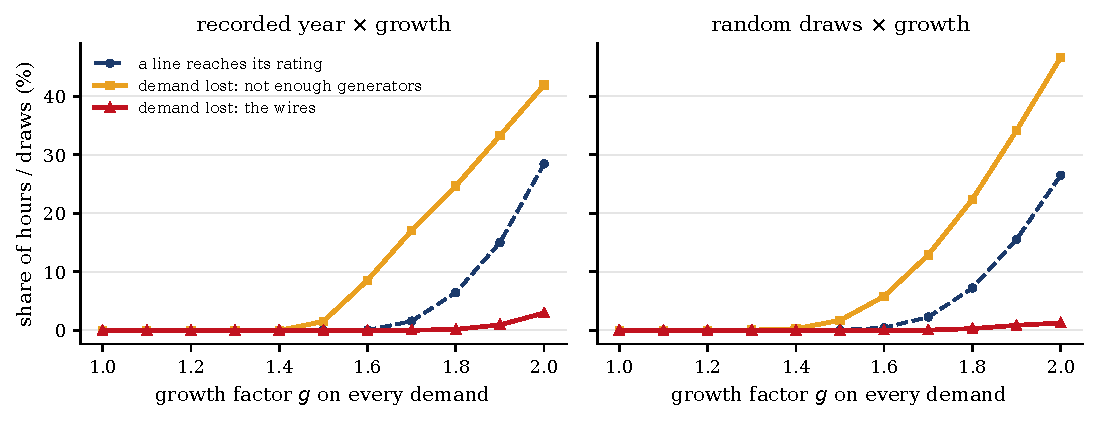
\includegraphics[width=\textwidth]{figs/fig5_growth.pdf}
\caption{\textbf{Every demand multiplied by $g$, every line in service.} Blue dashes:
share of hours (left) or draws (right) in which some line reaches its rating. Gold:
demand lost because the island's generators together are too small (it is lost even
with the line limits removed). Red: demand lost because of the wires alone (served when
the line limits are removed).}
\label{fig:growth}
\end{figure}

To separate a shortage of \emph{wire} from a shortage of \emph{generation}, every
growth case is solved twice: once as usual, and once with all line limits removed (a
``copper plate''). Demand lost in the copper plate is a generation shortage; demand
lost only when the limits are on is caused by the wires.

\begin{center}
\small
\begin{tabular}{@{}lcc@{}}
\toprule
\textbf{First happens at growth factor \dots} & \textbf{Recorded year} & \textbf{Random draws} \\
\midrule
generators too small in some hour (fleet \SI{1508}{MW})    & $g = 1.5$ & $g = 1.3$ \\
a line reaches its rating                                 & $g = 1.6$ & $g = 1.5$ \\
\quad \dots the lines: Waiau--Makalapa, Makalapa--Downtown & & \\
demand lost because of the wires                          & $g = 1.7$ & $g = 1.6$ \\
\quad \dots the areas: Pearl Harbor (Makalapa) and Downtown & & \\
\bottomrule
\end{tabular}
\end{center}

\Cref{fig:growth} shows the result: \textbf{with all lines in service, the recorded
year's demand can grow by \SI{40}{\percent} before anything runs short (the random
draws, with their longer tails, by \SI{20}{\percent}), and what runs short first is
generation, not wire.} Even at twice today's demand the wires alone cost
power in only \SI{3.0}{\percent} of recorded hours and \SI{1.3}{\percent} of random
draws, against \SI{42}{\percent} and \SI{47}{\percent} for the generators. The random
draws reach each threshold one or two steps earlier because their tails are longer. The Kalaeloa export pair
never reaches its rating under growth (CEIP--Ewa Nui peaks at \SI{95}{\percent} of it
in the recorded year and \SI{97}{\percent} in the random draws): its flow is set by the plants at Kalaeloa, which already deliver their
\SI{306}{MW} in every recorded hour and add only the last-resort CIP turbine as demand
grows.

\subsection{How much the answers depend on the stand-in numbers}
\label{sec:sens}

Two inputs are stand-ins with real uncertainty: the line ratings, and the split of
island demand between substations. Every outage case was re-run with each alternative.

\begin{table}[!htbp]
\centering
\small
\caption{\textbf{Sensitivity.} Recorded-year results (random draws in brackets) for
three per-circuit ratings and for the substation split re-weighted to the 2002 filed
shares (Pukele 17\%, Koolau 13\%, Downtown 25\%, rest in proportion)\src{PUC}.}
\label{tab:sens}
\footnotesize
\begin{tabular}{@{}lcccc@{}}
\toprule
& \textbf{150 MW} & \textbf{209.9 MW (base)} & \textbf{318.6 MW} &
  \textbf{209.9 MW,} \\
& \textbf{per circuit} & \textbf{per circuit} & \textbf{per circuit} &
  \textbf{2002 shares} \\
\midrule
N-0: highest loading & 100\% (100\%) & 73\% (73\%) & 48\% (48\%) & 74\% (75\%) \\
N-0: demand lost & never & never & never & never \\
N-1: cases that lose demand (of 16) & 4 (7) & 0 (0) & 0 (0) & 0 (1) \\
N-2: cases that lose demand (of 128) & 60 (91) & 7 (10) & 4 (4) & 6 (21) \\
\midrule
\multicolumn{5}{@{}l}{\textit{Share of hours short after the four key double outages}}\\
both Koolau--Pukele $\to$ East Honolulu & 100\% & 100\% & 100\% & 100\% \\
both Halawa--Downtown $\to$ Downtown & 100\% & 98.9\% & 12.6\% & 10.0\% \\
Kahe--Wahiawa + Wahiawa--Waiau $\to$ Wahiaw\=a & 36.8\% & 36.8\% & 36.8\% & 46.1\% \\
both Waiau--Koolau $\to$ Windward + E. Honolulu & 39.2\% & 7.9\% & 0\% & 45.9\% \\
\bottomrule
\end{tabular}
\end{table}

\Cref{tab:sens} separates what is robust from what is not.
\begin{itemize}
  \item \textbf{Robust:} no variant loses demand with every line in service. East
        Honolulu, downtown and Wahiaw\=a can lose power in every variant, and the
        windward side in all but the thickest-line one; Pearl Harbor joins only with
        the thinnest lines or in the random draws. East Honolulu's exposure does not
        depend on any stand-in at all: with no \SI{138}{kV} path left, the rating is
        irrelevant. Wahiaw\=a's depends only on the Schofield plant's size and
        Wahiaw\=a's demand.
  \item \textbf{Not robust:} how \emph{often} downtown and the windward side are
        short.
        Thicker lines (\SI{318.6}{MW}) cut downtown's exposure from \SI{99}{\percent}
        to \SI{13}{\percent} of hours and remove the windward one. The 2002 split moves
        load from downtown to the windward side and East Honolulu, and the two swap
        places: downtown falls to \SI{10}{\percent}, the windward side rises to
        \SI{46}{\percent}. (That variant gives the whole merged Downtown bus the 25\%
        filed for Iwilei and School Street alone, so it probably understates downtown.)
  \item \textbf{The \SI{150}{MW} rating is very unlikely for the real system.} With it,
        losing a single downtown circuit would leave downtown short in
        \SI{30}{\percent} of hours --- a failure of the utility's own single-outage
        rule that its 2021 study, which found ``no existing system equipment
        overloading issue''\src{REZ}, would not have missed.
\end{itemize}

\subsection{Local variation: does a full-rank $\Sigma$ change the answers?}
\label{sec:noise}

The demand table has no substation-specific variation, so its covariance matrix is
singular (\cref{sec:stats}). \Cref{tab:noise} repeats every outage test with the local
wiggle of \cref{eq:noise} at three sizes: $f = 0.10$, $0.25$ and $0.50$ of each
substation's own swing $\sigma_n$. Nobody publishes the right size --- it would take
metered substation data --- so these bracket it. Picture the cloud of demand vectors:
without the wiggle it is a flat three-dimensional sheet in a ten-dimensional room; the
wiggle gives it thickness in every direction.

\begin{table}[!htbp]
\centering
\small
\caption{\textbf{Adding local variation.} Recorded-year results, random draws in
brackets. $f$: size of each substation's independent wiggle as a share of its own
standard deviation. Thinnest direction: square root of the smallest eigenvalue of the
recorded-hour covariance matrix (zero means singular).}
\label{tab:noise}
\footnotesize
\begin{tabular}{@{}lcccc@{}}
\toprule
& $f = 0$ (base) & $f = 0.10$ & $f = 0.25$ & $f = 0.50$ \\
\midrule
\multicolumn{5}{@{}l}{\textit{What the wiggle does to the demand}}\\
thinnest direction of the demand cloud & \SI{0}{MW} & \SI{0.37}{MW} & \SI{0.94}{MW} & \SI{1.86}{MW} \\
average correlation between substations & 0.86 & 0.85 & 0.81 & 0.69 \\
Wahiaw\=a--Koolau correlation & 0.999 & 0.989 & 0.941 & 0.802 \\
spread of the island total, $\sigma$ & \SI{124.9}{MW} & \SI{125.0}{MW} & \SI{125.6}{MW} & \SI{127.6}{MW} \\
\midrule
\multicolumn{5}{@{}l}{\textit{What it does to the answers}}\\
N-0: demand lost & never & never & never & never \\
N-1: cases that lose demand (of 16) & 0 (0) & 0 (0) & 0 (0) & 0 (3) \\
N-2: cases that lose demand (of 128) & 7 (10) & 7 (11) & 8 (14) & 9 (37) \\
both Koolau--Pukele $\to$ East Honolulu & 100\% & 100\% & 100\% & 100\% \\
both Halawa--Downtown $\to$ Downtown & 98.9\% & 98.7\% & 98.0\% & 95.7\% \\
Kahe--Wahiawa + Wahiawa--Waiau $\to$ Wahiaw\=a & 36.8\% & 37.0\% & 37.9\% & 40.0\% \\
both Waiau--Koolau $\to$ Windward + E. Honolulu & 7.9\% & 8.0\% & 8.4\% & 8.6\% \\
1 Kahe--Halawa + 1 Waiau--Makalapa $\to$ Pearl Harbor & 0 h (33) & 0 h (36) & 1 h (44) & 15 h (65) \\
growth: generators first short at & $g=1.5$ (1.3) & & & $g=1.4$ (1.3) \\
growth: wires first cost demand at & $g=1.7$ (1.6) & & & $g=1.7$ (1.5) \\
\bottomrule
\end{tabular}
\end{table}

\begin{itemize}
  \item \textbf{The covariance becomes full rank, and the island barely notices.} The
        wiggles are independent, so across the island they mostly cancel: the island's
        spread rises by at most \SI{2.7}{MW}. What changes is how tightly substations
        move together --- at $f = 0.5$ Wahiaw\=a and Koolau are no longer near-copies
        (0.80 instead of 0.999).
  \item \textbf{The four at-risk areas and their order do not change.} No variant loses
        demand with every line in service, and no recorded hour loses demand after a
        single outage. The four areas' shortfall frequencies move by at most
        \SI{3.2}{percentage points}.
  \item \textbf{Pearl Harbor is the area that local variation exposes.} Makalapa, which
        hangs mostly off the two Waiau--Makalapa circuits, went short only in random
        draws before; with a wiggle of a quarter of its swing or more it goes short in
        recorded hours too (15 hours at $f = 0.5$).
  \item \textbf{The extra random-draw cases are rare.} Of the 37 double outages that
        lose demand in some draw at $f = 0.5$ (against 10 without the wiggle), 21 do so
        in only one or two of the \num{10000} draws --- mostly East Honolulu with one of
        its two circuits out, in a draw where Pukele alone rises above what one circuit
        carries.
\end{itemize}

%======================================================================
\section{Answers}
\label{sec:answers}
%======================================================================

\begin{center}
\small
\begin{tabular}{@{}p{0.27\textwidth}p{0.66\textwidth}@{}}
\toprule
\textbf{Question} & \textbf{Answer (base case; recorded year, random draws)} \\
\midrule
\textbf{How often can the network not supply the demand?} &
  With every line in service: \textbf{never} --- 0 of \num{8760} hours, 0 of
  \num{10000} draws. After any one circuit fails: never. After two circuits fail: in
  7 of the 128 possible pairs (10 in the random draws); in those, from one hour a year
  to every hour. \\[3pt]
\textbf{Which areas are most at risk?} &
  \textbf{1.~East Honolulu} (Pukele: Waik\=ik\=i, M\=anoa, Kaimuk\=i, K\=ahala,
  Hawai\okina i Kai) --- two circuits, one source; losing both cuts everything on the
  \SI{138}{kV} network. \textbf{2.~Downtown Honolulu} --- short in \SI{99}{\percent}
  of hours after losing two of its three feeders. \textbf{3.~Wahiaw\=a and the North
  Shore} --- islanded on the \SI{50}{MW} Schofield plant, short in \SI{37}{\percent}
  of hours (\SI{43}{\percent} of draws). \textbf{4.~The windward side with East
  Honolulu} --- short in \SI{8}{\percent} of hours (\SI{5}{\percent} of draws) after
  losing two of the three lines into Koolau. Pearl Harbor (Makalapa) is at risk in
  the random draws, under growth, and --- once each substation is given its own local
  variation --- in recorded hours too. \\[3pt]
\textbf{Which lines overload the most?} &
  \textbf{CEIP--Ewa Nui and Kalaeloa--Ewa Nui}, the two single circuits that carry the
  west side's power east (all of Kalaeloa's, part of Kahe's): the fullest lines in normal operation (\SI{73}{\percent}
  and \SI{68}{\percent}), and pinned at their rating in \SI{39}{\percent} and
  \SI{27}{\percent} of hours when the other one is out. Then the \textbf{downtown
  feeders}, whose overloads are the ones that end in lost demand. Under growth,
  \textbf{Waiau--Makalapa and Makalapa--Downtown} fill first (at $1.6\times$ demand). \\[3pt]
\textbf{Does random demand give the same answers as the recorded year?} &
  \textbf{Yes on every major finding} --- the same areas, the same lines, the same
  order, and frequencies within about six percentage points. The random draws add three
  rare failures (at most \SI{0.33}{\percent} of draws) that the recorded year never
  shows, and reach each growth threshold one or two steps earlier, because they include
  demands the year never had. They are more pessimistic about rare events, not about
  every row: the windward failure is \emph{less} frequent in the draws. \\
\bottomrule
\end{tabular}
\end{center}

The broad lesson is about \emph{shape}, not size. \Oahu's \SI{138}{kV} grid has
ample room in normal operation and survives any single failure. Its exposure is
concentrated in four places where a large load hangs off two or three circuits with no
plant of its own. Three of the four are the weaknesses the utility itself described to
its regulator in 2007\src{PUC}. The match is partly built in --- the circuit counts for
those areas come partly from the same order --- but the model adds what the order does
not give: how often, and by how much, each area would fall short on the \SI{138}{kV}
network.

%======================================================================
\section{Limitations}
\label{sec:limits}
%======================================================================

\begin{itemize}
  \item \textbf{Stand-in ratings and reactances.} The utility does not publish them.
        The reactance cancels out (\cref{sec:network}); the rating does not, and
        \cref{tab:sens} shows how far it moves the downtown and windward results.
  \item \textbf{No \SI{46}{kV} network.} Below \SI{138}{kV}, \Oahu{} has a
        \SI{46}{kV} network that can move some load between neighbouring substations ---
        the 2007 order approved exactly such ties for Pukele\src{PUC}. An area that
        ``loses power'' here might, in reality, lose part of it, or lose it only until
        switching is done.
  \item \textbf{Normal ratings for double outages.} The utility's rule allows emergency
        ratings after a second failure. Those are not published, so the N-2 results are
        pessimistic.
  \item \textbf{No metered substation data.} Hawaiian Electric does not publish hourly
        load by substation, so the substation split is built from census data by
        \cref{eq:demand}, and its shares differ from the only filed ones, from 2002
        (\cref{sec:stats}). Metered data would replace three stand-ins at once: the
        split, the correlations between substations, and each substation's own local
        variation. The local-noise runs (\cref{sec:noise}) only bracket how much the
        last one matters.
  \item \textbf{A three-factor demand.} Because every substation is a fixed mix of three
        island-wide sector curves, the substations move together more tightly than real
        ones do (correlations 0.47 to 1.00) and $\Sigma$ has rank three.
  \item \textbf{The industrial class.} Industry is \SI{42}{\percent} of the utility's 2021
        sales\src{EIA861} (\SI{51}{\percent} of net load after rooftop solar, which falls
        mostly on homes). It is given a flat daily shape and placed by industrial jobs;
        which large customers the class contains, and where they are, is not public.
  \item \textbf{The Gaussian is a summary.} It matches each substation's mean, spread and
        correlations, not its two-humped shape, and its tails reach demands the recorded
        year never had.
  \item \textbf{DC power flow, hour by hour.} Voltages, reactive power and losses are
        ignored, and each hour is solved on its own, with no start-up, minimum-output or
        ramping limits. Generator outages (the ``one generating unit on overhaul'' in
        the utility's rule) are not tested.
  \item \textbf{Fleet and year.} The fleet is the 2024 fossil and waste fleet; the demand
        is 2021's. Utility-scale solar, wind and batteries are not modelled, so the
        fleet must meet the whole net load alone.
\end{itemize}

%======================================================================
\section{Reproducing this}
%======================================================================

Every number in this paper is computed by the scripts in this folder, in this order,
and \texttt{check\_numbers.py} confirms that each number typed in the text matches
them.

\begin{center}
\small
\begin{tabular}{@{}lp{0.62\textwidth}@{}}
\toprule
\texttt{build\_network.py}    & substations, corridors, lengths, ratings (from HIFLD) \\
\texttt{build\_generators.py} & the 24 units, their bus and running cost \\
\texttt{build\_demand.py}     & hourly demand at each substation \\
\texttt{build\_demand\_puc.py}& the same, re-weighted to the 2002 filed shares \\
\texttt{run\_all.jl}          & N-0 on the recorded hours and the random draws;
                                Gaussian statistics \\
\texttt{contingency.jl}       & N-0, N-1 and N-2 (set \texttt{RATING=low|high},
                                \texttt{DEMAND=puc} or \texttt{NOISE=0.25} for the
                                sensitivities) \\
\texttt{stress.jl}            & the growth ladder (also with \texttt{NOISE}) \\
\texttt{noise\_stats.jl}      & what the local wiggle does to the demand inputs \\
\texttt{redispatch.jl}        & what the optimiser does when an export line is lost \\
\texttt{summarize.py}         & the numbers and tables in the text \\
\texttt{check\_numbers.py}     & recomputes the quoted numbers and checks the text \\
\texttt{makefigs.py}          & the five figures \\
\bottomrule
\end{tabular}
\end{center}

\noindent In total the runs solve \num{19930640} linear programs; every one returned a
proven optimum.

\appendix
%======================================================================
\section{Every input, and where it comes from}
\label{app:sources}
%======================================================================

\emph{Measured} means taken from a public record of \Oahu's own system.
\emph{Stand-in} means \Oahu's own value is not public, so the closest documented value
is used, and the text says what it stands in for.

\begin{small}
\begin{longtable}{@{}p{0.2\textwidth}p{0.2\textwidth}p{0.4\textwidth}p{0.1\textwidth}@{}}
\toprule
\textbf{Input} & \textbf{Value used} & \textbf{Source} & \textbf{Kind} \\
\midrule
\endhead
Substations and their locations & 11 buses & HIFLD transmission lines, line end points\src{HIFLD} & measured \\
Which substations are joined & 16 corridors & HIFLD\src{HIFLD}; single-line diagrams\src{REZ}; PUC order\src{PUC} & measured \\
Circuits per corridor & 1--3, 25 in all & \src{REZ} Figs.~30--36, Table 10-3; \src{RFP}; \src{AES}; \src{PUC}; HIFLD & measured \\
Line lengths & \SIrange{2.15}{20.69}{mi} & measured along HIFLD routes\src{HIFLD} & measured \\
Line reactance & \SI{0.48}{\ohm/km} & typical \SI{138}{kV} value\src{UT}; cancels from flows & stand-in \\
Per-circuit rating & \SI{209.9}{MW} & 795 AAC, as drawn for new \Oahu{} circuits\src{REZ}; \SI{878}{A}\src{SW} & stand-in \\
Rating, low & \SI{150}{MW} & $3\times$ SIL of a \SI{138}{kV} line\src{UT} & stand-in \\
Rating, high & \SI{318.6}{MW} & 1590 AAC, \src{REZ} Figs.~32, 34, 35; \SI{1333}{A}\src{SW} & stand-in \\
Power base & \SI{100}{MVA} & MATPOWER convention\src{MAT} & convention \\
Generating units, capacity & 24 units, \SI{1508.1}{MW} & EIA-860 2024, summer capacity\src{EIA860} & measured \\
Heat rates & per plant & EIA-923 2024\src{EIA923} & measured \\
Fuel prices & 2024 forecast & utility IGP Workbook~3\src{IGP} & utility forecast \\
Variable O\&M: CC, CT, engines & \$2, \$7, \$31/MWh & utility IGP, Tables A-9, A-10 (2024)\src{IGP} & stand-in (new units) \\
Variable O\&M: steam, waste & \$0.88, \$6.94/MWh & EPA Platform v6, Table 4-8 (2019\$)\src{EPA} & stand-in \\
H-Power fuel cost & \$0/MWh & burns municipal waste & assumption \\
Plant-to-substation map & 4 buses & own switchyards; \src{AES}; nearest substation & measured \\
Penalty for unserved demand & \$10{,}000/MWh & MISO value of lost load, FERC-accepted 2025\src{MISO} & stand-in \\
Island hourly load, 2021 & \num{8760} values & utility IGP Workbook~3\src{IGP} & measured (filed) \\
Population & 2020 tracts & U.S. Census 2020\src{CEN} & measured \\
Jobs & 2021 blocks & LEHD LODES8\src{LODES} & measured \\
Sector sales, PV and efficiency shares & 2021 & EIA-861\src{EIA861} & measured \\
Hourly shapes & homes, 15 building types & DOE reference buildings, Honolulu\src{OEI}; CBECS 2018\src{CBECS} & stand-in \\
Catchment rule & nearest substation & PyPSA-Eur\src{PYPSA}; Pukele list from \src{PUC} & method \\
Filed substation shares & 17\%, 30\%, 25\% & PUC order\src{PUC} (17\% and 25\% at the 2002 day peak) & filed (2002) \\
Local variation per substation & $f = 0.10, 0.25, 0.50$ of $\sigma_n$ & none published; metered substation load is not public & sensitivity \\
Coastline & 2020 shoreline & Census cartographic boundaries\src{CB} & measured \\
\bottomrule
\end{longtable}
\end{small}

%======================================================================
\section*{References}
%======================================================================
\begin{small}\sloppy
\begin{description}[leftmargin=4.2em,style=sameline,itemsep=2pt]
\item[{[AES]}] Hawaiian Electric, Application, Hawai\okina i PUC Docket No.\ 2016-0439
  (AES--CEIP 2 138\,kV line relocation), 30 Dec.\ 2016, pp.~1--2, 7.
  \url{https://www.hawaiianelectric.com/documents/about_us/investing_in_the_future/dkt_2016_0439_20161230_application_AES_CEIP_2_138_kV_OH_line_relocation.pdf}
\item[{[CB]}] U.S. Census Bureau, 2020 Cartographic Boundary File, county subdivisions,
  Hawai\okina i (\texttt{cb\_2020\_15\_cousub\_500k}).
  \url{https://www2.census.gov/geo/tiger/GENZ2020/shp/cb_2020_15_cousub_500k.zip}
\item[{[CBECS]}] U.S. EIA, Commercial Buildings Energy Consumption Survey 2018, Tables
  C22 and B1. \url{https://www.eia.gov/consumption/commercial/data/2018/}
\item[{[CEN]}] U.S. Census Bureau, 2020 Census tracts and county subdivisions, Honolulu
  County (TIGERweb, Census 2020 layers 6 and 20).
  \url{https://tigerweb.geo.census.gov/arcgis/rest/services/TIGERweb/tigerWMS_Census2020/MapServer}
\item[{[EIA860]}] U.S. EIA, Form EIA-860, 2024 final data.
  \url{https://www.eia.gov/electricity/data/eia860/}
\item[{[EIA861]}] U.S. EIA, Form EIA-861, 2021 (sales, net metering, distributed
  generation, energy efficiency). \url{https://www.eia.gov/electricity/data/eia861/}
\item[{[EIA923]}] U.S. EIA, Form EIA-923, 2024 final data.
  \url{https://www.eia.gov/electricity/data/eia923/}
\item[{[EPA]}] U.S. EPA, Power Sector Modeling Platform v6 (Summer 2021 Reference Case),
  Documentation Chapter~4, Table 4-8.
  \url{https://www.epa.gov/system/files/documents/2021-09/chapter-4-generating-resources.pdf}
\item[{[GEG]}] K.~M.~Gegner, A.~B.~Birchfield, T.~Xu, K.~S.~Shetye, T.~J.~Overbye,
  ``A methodology for the creation of geographically realistic synthetic power flow
  models,'' \emph{IEEE Power and Energy Conference at Illinois}, 2016, Sec.~IV.A.
\item[{[HIFLD]}] U.S. DHS/CISA, Homeland Infrastructure Foundation-Level Data, ``Electric
  Power Transmission Lines'' feature service, queried for \Oahu{} on 22 Sept.\ 2026.
  \url{https://services1.arcgis.com/Hp6G80Pky0om7QvQ/arcgis/rest/services/Electric_Power_Transmission_Lines/FeatureServer/0}
\item[{[IGP]}] Hawaiian Electric, \emph{2021 Integrated Grid Planning Inputs and
  Assumptions}, Aug.\ 2021 update, Tables A-9 and A-10, pp.~A-10--A-11; and Final
  \Oahu{} IGP Inputs Workbook~3, filed 31 Mar.\ 2022.
  \url{https://www.hawaiianelectric.com/documents/clean_energy_hawaii/integrated_grid_planning/stakeholder_engagement/working_groups/forecast_assumptions/20210818_finaligp_inputs_and_assumptions.pdf};
  \url{https://www.hawaiianelectric.com/documents/clean_energy_hawaii/integrated_grid_planning/20220331_final_oahu_inputs_workbook_3_revised.xlsx}
\item[{[LODES]}] U.S. Census Bureau, LEHD Origin-Destination Employment Statistics
  (LODES8), Hawai\okina i, 2021 workplace area characteristics.
  \url{https://lehd.ces.census.gov/data/lodes/LODES8/hi/}
\item[{[MAT]}] R.~D.~Zimmerman, C.~E.~Murillo-S\'anchez, R.~J.~Thomas, ``MATPOWER:
  Steady-state operations, planning, and analysis tools for power systems research and
  education,'' \emph{IEEE Trans.\ Power Systems} 26(1):12--19, 2011.
\item[{[MISO]}] RTO Insider, ``FERC approves MISO value of lost load increase'' (value
  of lost load raised from \$3{,}500 to \$10{,}000/MWh), 2025.
  \url{https://www.rtoinsider.com/102108-ferc-approves-miso-value-lost-load-increase/};
  MISO Market Subcommittee, ``Continued reforms to improve scarcity pricing,'' 21 Aug.\ 2025.
\item[{[OEI]}] OpenEI / U.S. DOE, Commercial and Residential Hourly Load Profiles for all
  TMY3 Locations (Honolulu Intl.\ AP). \url{https://openei.org/datasets/files/961/pub}
\item[{[PUC]}] Hawai\okina i Public Utilities Commission, Decision and Order No.~23747,
  Docket No.~03-0417 (East \Oahu{} Transmission Project), 2007, pp.~7--11.
  \url{https://files.hawaii.gov/dcca/dca/dno/dno2007/23747.pdf}
\item[{[PYPSA]}] J.~H\"orsch, F.~Hofmann, D.~Schlachtberger, T.~Brown, ``PyPSA-Eur: An
  open optimisation model of the European transmission system,'' \emph{Energy Strategy
  Reviews} 22:207--215, 2018, Secs.~2.1 and 2.6.
\item[{[REZ]}] Hawaiian Electric, \emph{Transmission Renewable Energy Zone Study}, Nov.\
  2021, Sec.~5.4, Table 5-3, Figs.~30--36.
  \url{https://www.hawaiianelectric.com/documents/clean_energy_hawaii/integrated_grid_planning/stakeholder_engagement/working_groups/solution_evaluation_and_optimization/20211105_transmission_renewable_energy_zone_study.pdf}
\item[{[RFP]}] Hawaiian Electric, IGP RFP for Renewable Dispatchable Generation and
  Energy Storage (\Oahu{} and Hawai\okina i Island), Appendix~H, Attachment~1, p.~1
  (worked example).
  \url{https://www.hawaiianelectric.com/documents/clean_energy_hawaii/selling_power_to_the_utility/competitive_bidding/igp_rfp/igp_rfp_appx_h_interconnection_facilities_cost_and_schedule.pdf}
\item[{[SW]}] Southwire, AAC bare aluminium conductor, specification 80120, Table~2.
  \url{https://cabletechsupport.southwire.com/en/cablespec/download_spec/?spec=80120}
\item[{[UT]}] University of Utah, ECE 3600 lecture notes, ``Transmission Lines'', table
  ``Transmission Line Typical Values''.
  \url{https://my.ece.utah.edu/~ece3600/Notes_TransmissionLines_S23.pdf}
\end{description}
\end{small}

\end{document}
